\addcontentsline{toc}{chapter}{Appendix - Résumé en français}
\chapter*{Appendix - Résumé en français}
\markboth{\MakeUppercase{Appendix - Résumé en français}}{}

\addcontentsline{toc}{section}{Introduction}
\section*{Introduction}
%Over the past decade, we have witnessed a dramatic increase in the number of social Web applications. These applications come in different forms and offer different services such as social networks, content management systems (CMS), software forges, bug trackers, blogging tools, or collaboration services in general.\\
Au cours de la dernière décennie, nous avons assisté à une augmentation spectaculaire du nombre d'applications Web sociales. Ces applications sont disponibles en différentes formes et offrent différents services comme les réseaux sociaux, les systèmes de gestion de contenu (CMS), les forges logicielles, les blogs ou les services de collaboration en général.\\


%Since the launch of the first large social networking website in 1997~\cite{ellison2007social}, the social Web has seen a significant increase in its size and usage. Rather than simply consuming websites, users began to generate their own content through blogging tools and social networks, marking the start of Web 2.0 and the Semantic Web~\cite{berners1999weaving}. Social Websites responded to this new trend by providing users with the ability to create their own personal profile where they could list friends, post photos, status updates and more. Later, some of these websites also provided plug-ins that were used to integrate some of their social functionalities on third-party websites. But what exactly is a social website and what functionalities do these websites offer to users? Is the ability to form a connection between users enough to consider a website to be a part of the social Web, and how can we expect the social Web to evolve in the future?\\
Depuis le lancement du premier grand site de réseau social en 1997~\cite{ellison2007social}, le Web social a vu une augmentation significative de sa taille et de son utilisation. Plutôt que de simplement consommer des sites Web, les utilisateurs ont commencé à produire leurs propres contenus grâce à des outils de blogging et des réseaux sociaux, marquant le début du Web 2.0 et du Web sémantique~\cite{berners1999weaving}. Les sites sociaux ont réagi à cette nouvelle tendance en offrant aux utilisateurs la possibilité de créer leur propre profil personnel, où ils peuvent publier des photos, mettre à jour leur statut ou bien plus. Plus tard, certains de ces sites ont également fourni des plug-ins qui ont été utilisés pour intégrer certaines de leurs fonctionnalités sociales sur des sites tiers. Mais qu'est-ce exactement un site de réseau social et quelles fonctionnalités ont ces sites à offrir aux utilisateurs? Est-ce que la capacité à former une connexion entre les utilisateurs est suffisante pour dire qu'un site fait partie du Web social? Que pouvons-nous attendre du Web social dans l'avenir?\\


%In this thesis we will analyse and propose means to achieve data ownership and interoperability for the next-generation social Web applications, with respect to privacy and access control. Our contributions concern different topics, from identity and authentication to access control and personal data storage.
Dans cette thèse, nous allons analyser et proposer des moyens d'assurer la propriété des données et l'interopérabilité des applications Web sociales de la prochaine génération, en ce qui concerne la vie privée et le contrôle d'accès. Nos contributions portent sur différents sujets, de l'identité et de l'authentification décentralisée au contrôle d'accès et le stockage des données personnelles.

\addcontentsline{toc}{subsection}{Motivation}
\subsection*{Motivation}
%A current practice of most Web services is to centralize user resources, becoming the so-called "data silos". Often when adhering to particular services we usually end up creating dedicated local accounts, which ties and limits us to a particular service and/or resource. Furthermore, users have no control over how their personal account data are used by applications, as it is the case for private data that is often sent to third party companies for advertising purposes.\\
Une pratique courante spécifique à la plupart des services Web est de centraliser les ressources utilisateurs, devenant des «silos de données». Souvent, lors de son adhésion à des services particuliers, nous finissons généralement par créer des comptes locaux dédiés qui nous limite à un service particulier. De plus, les utilisateurs n'ont aucun contrôle sur la façon dont leurs données personnelles sont utilisées par les applications, comme c'est le cas pour les données privées qui sont souvent envoyés à des sociétés tiers afin de réaliser des gains publicitaires.\\


%Identity is easily one of the most difficult research areas on the Web, as it requires both practical solutions and multidisciplinary research. We believe that identity implies to be able to refer reliably to anything, abstract or more concrete, over time and space, and in different contexts. One way to deal with identity is to establish a common convention that identifies particular things in a uniform manner that is easily reused in diverse contexts. When applied to the Web, it becomes obvious that using HTTP Uniform Resource Identifiers (URIs) as global identifiers is the preferred choice. The key advantage of HTTP URIs over any other identification scheme (e.g. email addresses, unique user IDs, etc.) is that linked data principles say these URIs should return a useful description of what the URI identifies when accessed in a Web browser or computer application using the HTTP protocol.\\
L'identité est l'un des domaines de recherche les plus difficiles sur le Web, car il nécessite à la fois des solutions pratiques et de la recherche multidisciplinaire. Nous croyons que l'identité implique de pouvoir se référer à quoi que ce soit de manière fiable, abstraite ou plus concrète, sans contraintes de temps et d'espace, et dans des contextes différents. Une façon de traiter le sujet de l'identité est d'établir une convention commune qui identifie des choses particulières d'une manière uniforme, et qui est facilement réutilisée dans différents contextes. Lorsqu'on l'applique sur le Web, il devient évident que l'utilisation des URI (Uniform Resource Identifiers) HTTP comme identificateurs globaux est le choix préféré. Le principal avantage des URI HTTP sur n'importe quel autre système d'identification (e.g. les adresses électroniques, ou bien les noms d'utilisateur uniques) est que les principes de données liées disent que ces URI doit retourner une description utile de ce que l'URI identifie lors de l'accès aux données dans un navigateur Web ou dans une application informatique en utilisant le protocole HTTP.\\



%A decentralized Web application must be able to function \textbf{across different application domains}, enabling different applications to interact with each other through the use of data semantics. It is important that users be allowed to choose where to store their data, may that be on personal servers they own and keep in their homes, entrusting their data to their friends or people they trust. Users may even take advantage of a myriad of cloud storage services available on the Web, though steps must be taken to ensure the privacy of their data, with respect to the service providers. To achieve true interoperability, we have decided to use the Semantic Web, as means to provide structured data that can also be understood by machines.\\
Une application Web décentralisé doit être capable de fonctionner à travers différents domaines d'application, ce qui permet aux différentes applications d'interagir les unes avec les autres grâce à l'utilisation des données sémantique. Il est important que les utilisateurs ont la possibilité de choisir où stocker leurs données, que ce soit sur des serveurs personnels qu'ils détiennent dans leurs maisons, ou en confiant leurs données à leurs amis ou des personnes de confiance. Les utilisateurs peuvent même profiter d'une myriade de  services de stockage de type «cloud» disponibles sur le Web, même si des mesures doivent être prises pour assurer la confidentialité de leurs données en ce qui concerne les prestataires de services. Pour atteindre une véritable interopérabilité, nous avons décidé d'utiliser le Web sémantique en tant que moyen pour fournir des données structurées qui peut aussi être comprise par les machines.\\


%The Semantic Web should be considered in some ways like a global database, or better yet an information space. Since most of the information on the Web is designed for human readers, though only useful for human-to-human interaction, the Semantic Web intends to allow machines to participate in this interaction by providing languages for expressing information in a machine processable form. In other words, the Semantic Web offers the tools to convey the meaning of data so that it will be understood by computers and not misinterpreted.\\
Le Web sémantique doit être considérée en quelque sorte comme une base de données globale, ou mieux encore un espace d'information global.  Puisque la plupart des informations sur le Web sont conçues pour les humains, dans des interactions homme-à-homme, le Web sémantique a l'intention de permettre aux machines de participer à cette interaction en fournissant des langages pour exprimer les informations sous des formes traitable par les machines. Autrement dit, le Web sémantique offre les outils nécessaires pour exprimer aussi ce que signifie les données afin qu'elles soient comprises et interprétées par des ordinateurs.\\


%The most common means used by the Semantic Web to describe information are the Resource Description Framework (RDF)~\cite{klyne2004resource} and Turtle~\cite{beckett2008turtle}. They are based upon the idea of making statements about resources (in particular Web resources) in the form of subject-predicate-object expressions, which are called \textit{triples}. The Semantic Web facilitates cross-domain applications and services, thanks to data being structured in ontologies and vocabularies. An ontology formally represents knowledge as a set of concepts within a domain, and the relationships between those concepts. Vocabularies are a less formal way of expressing concepts or entities and the relations between them.\\
Les moyens les plus couramment utilisées par le Web sémantique pour décrire l'information sont le RDF~\cite{klyne2004resource} (Resource Description Framework) et la syntaxe Turtle~\cite{beckett2008turtle}. Ils sont basés sur le concept de faire des déclarations au sujet des ressources (en particulier les ressources Web) sous la forme d'expressions sujet-prédicat-objet, qui sont appelés \textit{triples}. Le Web sémantique facilite les applications et les services inter-domaines, grâce aux données qui sont structurées en ontologies et vocabulaires. Une ontologie représente officiellement la connaissance comme un ensemble de concepts dans un domaine, et les relations entre ces concepts. Les vocabulaires sont une manière moins formelle d'exprimer des concepts ou des entités et les relations entre eux.

\addcontentsline{toc}{section}{Identité et authentification sur le Web}
\section*{Identité et authentification sur le Web}
%Identity is a complex concept, reflecting issues of stability, context, privacy and ownership, across real and virtual media. The goal of identity assurance, together with the consequences that follow when identity cannot be assured, has become the focus of significant research efforts.\\
L'identité est un concept complexe, réfléchissant aux questions de contexte, de vie privée et de propriété, à travers les médias réels et virtuels. Le but de l'assurance de l'identité, ainsi que les conséquences qui en découlent lorsque l'identité ne peut être assurée, est devenu un centre important des efforts de recherche.\\


%Decentralized, user-centric identity management offers better privacy and control over the use of identity credentials, since it allows users to flexibly choose what identity information is released to other entities in each transaction. For instance, users may choose to use a trusted Identity Provider (IdP) that they believe is the most appropriate for each transaction, or they may even use their own identity provider, therefore allowing them to control what identity information is disclosed to Service Providers (SP).\\
La gestion de l'identité décentralisée mais centrée sur l'utilisateur offre une meilleure protection des donnees personnels et de contrôle sur l'utilisation des informations d'identité, car elle permet aux utilisateurs de choisir de manière flexible les informations d'identité qui sont transmises à d'autres participants dans chaque transaction.\\

\addcontentsline{toc}{subsection}{Identité décentralisée avec WebID}
\subsection*{Identité décentralisée avec WebID}
%A global distributed Social Web requires that each person be able to control their identity and that this identity be linkable across sites, thus placing each person in a Web of relationships.\\
Un Web social distribué mondiale exige que chaque personne soit en mesure de contrôler leur identité et que cette identité est linkable à travers les sites, plaçant donc chaque personne dans un réseau de relations.\\


%WebID~\cite{webid2013}, our first contribution, is a simple and universal identification mechanism that is distributed, openly extensible, improves privacy, security and control over how each person can identify themselves in order to allow fine grained access control to their information on the Web. It does this by applying the best practices of Web Architecture whilst building on well established widely deployed protocols and standards including HTML~\cite{berners1995hypertext}, URIs~\cite{berners1998uniform}, HTTP~\cite{berners1996hypertext}, and RDF semantics. WebID is a work-in-progress open standard within the World Wide Web Consortium\footnote{http://w3.org}, to which we are actively contributing.\\
WebID, notre première contribution, est un mécanisme d'identification simple et universel qui est distribué, ouvertement extensible, améliore la confidentialité, la sécurité et le contrôle sur la façon dont chaque personne peut s'identifier, afin de permettre le contrôle d'accès à leur information sur le Web. Cela se fait en appliquant les meilleures pratiques de l'architecture du Web, tout en s'appuyant sur des protocoles et des normes largement déployées et bien établis, y compris HTML~\cite{berners1995hypertext}, les URI~\cite{berners1998uniform}, HTTP~\cite{berners1996hypertext}, et RDF. WebID est un standard ouvert au sein du World Wide Web Consortium, auquel nous contribuons activement.\\


%The general idea behind WebID is that Agents (e.g. a person, an organization, a group, etc.) create their own identities by linking a \textit{unique identifier} (i.e. an HTTP URI) to a \textit{profile document}, a type of Web page that any Web user is familiar with, and which uses a standardized RDF serialization format. The profile document contains all the necessary information to create a Web of trust which allows people to link together their profiles in a public or protected manner. Such a Web of trust can then be used by Web services to make authorization decisions, by allowing access to resource depending on the properties of an agent, such that he/she is known by some relevant people, works at a given company, is a family member, is part of some group, etc..\\
L'idée générale derrière WebID est que les agents (par exemple, une personne, une organisation, un groupe, etc) créent leurs propres identités en associant un \textit{identifiant unique} (un URI HTTP) à un \textit{document de profil}, un type de page Web que tout Web utilisateur est familiarisé avec, et qui utilise un format de sérialisation RDF standardisé. Le document de profil contient toutes les informations nécessaires pour créer un Web de confiance qui permet aux gens de faire le lien entre leurs profils de manière publique ou protégée. Un tel réseau de confiance peut alors être utilisé par les services Web pour prendre des décisions d'autorisation, en permettant l'accès aux ressources en fonction des propriétés d'un agent, tel qu'il est connue par certaines personnes concernées, travaille dans une entreprise donnée, est une membre de la famille, fait partie d'un groupe, etc.\\

%To exemplify these terms, Figure~\ref{fig:webid} describes the relations between Tim Berners-Lee's WebID (i.e. the URI) and the profile document to which it refers.\\
Pour illustrer ces termes, la Figure~\ref{fig:webid_fr} décrit les relations entre le WebID de Tim Berners-Lee (l'URI) et le document de profil auquel il se réfère.

\begin{figure}[h]
  \begin{center}
    \includegraphics[width=350px]{img/WebID-overview.png}
        \caption{La relation entre la personne (Tim Berners-Lee), le WebID (http://www.w3.org/People/Berners-Lee/card\#i) et le document de profil (http://www.w3.org/People/Berners-Lee/card).}
        \label{fig:webid_fr}
  \end{center}
\end{figure}


\subsubsection{URI WebID}
%On the Semantic Web, URIs identify not just Web documents, but also real-world objects like people and cars, and even abstract ideas and non-existing things like mythical heroes. We can refer to these as real-world objects or things. For example, the person Ann is described on her homepage. Barry may not like the look of the homepage, but may want to link to the person Ann. Therefore, two URIs are needed, one for Ann, one for the homepage or an RDF document describing Ann.\\
Dans le Web sémantique, les URI servent à identifier non seulement des documents Web, mais aussi des objets du monde réel comme des personnes, des voitures, et même des idées abstraites et des choses qui n'existent pas (comme des héros mythiques). Nous pouvons nous référer à eux comme à des objets ou des choses du monde réel. Par exemple, la personne Ann est décrite sur sa page d'accueil. Barry peut ne pas vouloir mettre un lien vers la \textit{page d'accueil} d'Ann, mais peut vouloir lier à la \textit{personne} Ann. Par conséquence, deux URI sont nécessaires, un pour Ann et un pour la page d'accueil ou un document RDF décrivant Ann.\\


%The main reason why fragment identifiers, commonly known as hashes (i.e. \#me), were introduced is that the WebID URI and the profile document URI should not be the same. If they were the same, then there would be no way to differentiate between the profile document's URI - https://barry.example/profile - and the URI pointing to the profile graph within the document (i.e. \textit{\#me}), which describes the user. In other words, for hash WebIDs, the URI without the hash denotes the \textit{profile document}.\\
La raison principale pour laquelle les identifiants de fragments, communément appelés hashes (i.e. \#me), ont été introduites, c'est que l'URI du WebID et l'URI du document de profil ne devraient pas être les mêmes. Si elles étaient les mêmes, il n'y aurait aucun moyen de différencier entre l'URI du document de profil - https://barry.example/profile - et l'URI pointant vers le graphe du profil qui décrit l'utilisateur dans le document (i.e. \#me). Autrement dit, pour les WebIDs avec des hashes, l'URI sans le hash indique le \textit{document de profil}.\\

%However, if hash URIs cannot be utilized, then an HTTP request on the WebID must return an HTTP 303 response with a \textit{Location} header URI referring to the profile document. Hash URIs are encouraged when choosing a WebID since HTTP 303 redirects impact performance for clients by means of additional requests. From here on, all examples will contain such hash URIs.
Toutefois, si des URIs hash ne peut pas être utilisé, alors une requête HTTP GET sur le WebID doit renvoyer une réponse HTTP 303 avec un URI dans l'emplacement en-tête se référant au document de profil. Les URI hash sont encouragés lors du choix d'un WebID, car les redirections HTTP 303 générer des demandes supplémentaires et ont un impact sur les performances pour les clients.

\subsubsection*{Le document de profil WebID}
%Personal details are the most common requirement when registering an account with a website. Some of these pieces of information include an e-mail address, a name and perhaps an image depicting the user. To this regard, WebID profiles are built using vocabularies identified by URIs (such as FOAF~\cite{foaf}, SIOC~\cite{breslin2005towards}, DOAP~\cite{dumbill2012doap}, etc.), that can be placed in subject, predicate or object position of the relations constituting an RDF graph. The definition of each URI is found at the namespace of the URI, by dereferencing it. For example, a \textbf{foaf:name} relation implies that the \textit{foaf:} namespace has been previously defined as a prefix in the following way: \textit{@prefix foaf: <http://xmlns.com/foaf/0.1/>}.\\
Les données personnelles sont l'exigence la plus courante lors de l'enregistrement d'un compte sur un site Web. Certains de ces éléments d'information contenant une adresse e-mail, un nom et peut-être une image représentant l'utilisateur. Pour ce qui concerne les profils WebID, ils sont construits en utilisant des vocabulaires identifiés par des URI (tels que FOAF~\cite{foaf}, SIOC~\cite{breslin2005towards}, DOAP~\cite{dumbill2012doap}, etc), qui peut être placé dans la position du sujet, prédicat ou objet des relations constituant un graphe RDF. La définition de chaque URI est obtenue par déréférencement de l'espace de noms de l'URI. Par exemple, un relation de type \textit{foaf:name} implique que le préfixe \textit{foaf:} a été précédemment définie comme un espace de noms de la façon suivante: \textit{@ prefix foaf: <http://xmlns.com/foaf/0.1/>}.\\


%A notable advantage of WebID over other identity schemes is that WebID can be easily extended. By simply expressing different information through additional vocabularies, WebID profile documents have the useful characteristic that they can be easily merged, allowing partial and decentralized descriptions to be combined in interesting ways. In WebID profile documents, additional vocabularies can be used either to extend the user's personal profile, by means of providing location coordinates, a list of personal interests and more, as well as to describe different activities related to the user - e.g. the user's blog posts, projects to which he/she contributes, etc.\\
Un avantage notable de WebID sur les autres systèmes d'identité est que WebID peut être facilement étendu. Dans les documents de profil WebID, des vocabulaires supplémentaires peuvent être utilisés pour étendre le profil personnel de l'utilisateur, par des moyens de fournir les coordonnées GPS, une liste des intérêts personnels, ainsi que décrire des différentes activités liées à l'utilisateur - par exemple son blog, les projets auxquels l'utilisateur contribue, etc.

\addcontentsline{toc}{subsection}{Authentification décentralisée avec WebID-TLS}
\subsection*{Authentification décentralisée avec WebID-TLS}
%Our second contribution, the WebID-TLS authentication protocol~\cite{webid-tls}, enables secure, efficient and user friendly authentication on the Web by allowing people to choose a client certificate proposed to them by their browser during the authentication process. A very important aspect of WebID-TLS is that it replaces standard username-password authentication methods, At the same time, it is easy to implement since it takes advantage of the cryptography behind the Transport Layer Security (TLS) protocol~\cite{dierks2008transport}. Furthermore, it is not affected by the same issues that are common to PKIs, since it does not rely on Certificate Authorities. Using self-signed certificates also means reducing costs created from issuing certificates by trusted CAs.\\
Notre deuxième contribution, le protocole d'authentification WebID-TLS~\cite{webid-tls}, permet une authentification efficace et facile à utiliser sur le Web en permettant aux utilisateurs de choisir un certificat client proposé par leur navigateur au cours du processus d'authentification. Un aspect très important de WebID-TLS, c'est qu'il remplace les méthodes d'authentification standard basés sur les noms d'utilisateur et mots de passe. En même temps, il est facile à mettre en œuvre car il tire parti de la cryptographie derrière le protocole de sécurité de la couche transport (TLS)~\cite{dierks2008transport}. En outre, il n'est pas affecté par les mêmes problèmes qui sont communs à IPK, car il ne repose pas sur les autorités de certification. Utiliser des certificats auto-signés c'est aussi réduire les coûts créés à partir de la délivrance des certificats signés par des autorités de certification.\\


%The main advantage of WebID-TLS is the fact that it is a truly decentralized authentication protocol, with no pre-existing trust relationships required between the SP and the IdP. In WebID-TLS, trust is built by using the Semantic Web to imaginatively reason over the contents of the profile document.\\
Le principal avantage de WebID-TLS est le fait qu'il s'agit d'un protocole d'authentification véritablement décentralisé, sans relations de confiance préexistantes nécessaires entre le fournisseur de services (SP) et le fournisseur d'identité (IdP). Dans WebID-TLS, la confiance se construit en utilisant le Web sémantique pour raisonner sur le contenu du document de profil.\\


%In order to provide the full context of a user/agent authentication to a service provider we will illustrate the protocol with the following sequence diagram (cf. Figure~\ref{fig:webid-flow}). It should be noted that from a user's point of view, the complete process of WebID-TLS authentication is simply a one click operation in which he/she chooses the WebID certificate. The user is not required to remember any credentials in order to authenticate.
Afin de fournir le contexte global d'une authentification de l'utilisateur ou d'un agent à un prestataire de services, nous allons illustrer le protocole avec le diagramme de séquence suivante (cf. Figure~\ref{fig:webid-flow-fr}). Il faut noter que du point de vue de l'utilisateur, le processus complet d'authentification WebID-TLS est tout simplement \textit{un clic} qui permet de choisir le certificat WebID. L'utilisateur n'est pas obligé de se rappeler les informations d'identification pour s'authentifier.\\

\begin{figure}[h]
  \begin{center}
    
\includegraphics[width=200px]{img/webid.pdf}
        \caption{Le flux d'authentification WebID-TLS.}
        \label{fig:webid-flow-fr}
  \end{center}
\end{figure}

%The steps involved in the WebID-TLS authentication flow are as follows:
Les étapes impliquées dans le flux d'authentification WebID-TLS sont les suivantes:

\begin{enumerate}
\item Tout en essayant d'accéder à une ressource protégée sur le SP, l'utilisateur est invité à fournir un certificat client, dans le cadre de la négociation TLS. À ce stade, le SP vérifie que l'utilisateur possède la clé privée correspondant à la clé publique du certificat envoyé au SP.
\item Le vérificateur WebID de SP extrait le URI du WebID de l'extension \textit{SubjectAlternativeName} situé dans le certificat d'utilisateur, ainsi que le module et l'exposant correspondant à la clé publique du certificat.
\item Le vérificateur WebID récupère le document de profil WebID de l'IdP pour obtenir les clés publiques de l'utilisateur contenant les modules et les exposants.
\item Le vérificateur WebID vérifie si les éléments de la clé publique (i.e. module et exposant) du certificat de l'utilisateur correspondent aux éléments de la clé publique figurent dans le document de profil WebID. Si elles correspondent, l'utilisateur est alors authentifié avec succès sur le SP.
\end{enumerate}

\addcontentsline{toc}{subsection}{L'authentification déléguée pour WebID-TLS}
\subsection*{L'authentification déléguée pour WebID-TLS}
%WebID-TLS delegated authentication is the process of using a third-party authentication service in cases where Web applications and services either do not offer TLS or DANE~\cite{hoffman2012dns} capabilities, or choose not to host the WebID verifier service themselves. WebID-TLS delegated authentication adds another entity to the authentication flow, namely the Relying Party (RP), as seen in Figure~\ref{fig:webid-relying}.\\
L'authentification déléguée WebID-TLS est le processus d'utilisation d'un service d'authentification tiers dans les cas où des applications Web ou les services ne peuvent pas fonctionner sur TLS, ou choisissent de ne pas héberger le service vérificateur WebID eux-mêmes. L'authentification déléguée WebID-TLS ajoute une autre entité au flux d'authentification, qui est la partie de confiance (RP), comme on le voit dans la Figure~\ref{fig:webid-relying-fr}.\\


\begin{figure}[h]
  \begin{center}
    \includegraphics[width=200px]{img/webid-relying.pdf}
        \caption{Le flux d'authentification déléguée WebID-TLS.}
        \label{fig:webid-relying-fr}
  \end{center}
\end{figure}

%The steps involved in the WebID-TLS delegated authentication flow are as follows:
Les étapes impliquées dans le flux d'authentification déléguée WebID-TLS sont les suivantes:\\

\begin{enumerate}
\item Contrairement à l'authentification WebID-TLS standard, dans ce cas, l'utilisateur est d'abord redirigé vers un service vérificateur de WebID tiers, le RP.
\item Le vérificateur WebID de SP extrait le URI du WebID de l'extension \textit{SubjectAlternativeName} situé dans le certificat d'utilisateur, ainsi que le module et l'exposant correspondant à la clé publique du certificat.
\item Le vérificateur WebID récupère le document de profil WebID de l'IdP pour obtenir les clés publiques de l'utilisateur contenant les modules et les exposants.
\item Le vérificateur WebID vérifie si les éléments de la clé publique (i.e. module et exposant) du certificat de l'utilisateur correspondent aux éléments de la clé publique figurent dans le document de profil WebID. Si elles correspondent, l'utilisateur est alors authentifié avec succès sur le RP.
\item Le RP redirige l'utilisateur vers le SP, ajoutant des informations supplémentaires afin d'attester l'identité de l'utilisateur, ainsi que d'une signature pour prouver l'authenticité du message - c'est à dire le message provient d'un vrai RP et non d'un attaquant.
\item Le SP vérifie la signature ci-dessus et connecte l'utilisateur dans l'application, tandis que dans le même temps il récupère les données sur l'utilisateur à partir de son IdP.
\end{enumerate}

\addcontentsline{toc}{subsection}{Délégation d'accès pour WebID-TLS}
\subsection*{Délégation d'accès pour WebID-TLS}
%It is worth noting that the host serving WebID profiles controls the identity of every agent whose URI is within that server's domain. This host is known as the origin server, and it is the origin of all resources served by it. We can easily think of the origin server as not only able to respond to requests, but also as an agent able to make requests. Indeed, WebID-TLS authentication requires the server to make WebID profile requests to other servers in order to verify the identity of agents making a request to it. The WebID specification describes this task as being accomplished by a separate agent, the WebID verifier - which could indeed be done by another service on the web (i.e. WebID relying parties or proxy authentication servers). The WebID profile furthermore could be served by the same agent as the one making the request, in which case we have a minimal case of a peer to peer communication.\\
Il faut noter que le serveur hébergeant les profils WebID contrôle l'identité de chaque agent dont l'URI est dans le domaine de ce serveur. Cet hôte est connu comme le serveur d'origine, et il est à l'origine de toutes les ressources qu'il dessert. Nous pouvons facilement imaginer le serveur d'origine, non seulement en mesure de répondre aux demandes, mais aussi comme un agent capable de faire des demandes. Un vérificateur WebID-TLS nécessite que son propre serveur fait des demandes pour les profils WebID vers d'autres serveurs pour chercher le document de profil de l'utilisateur demandeur. La spécification WebID décrit cette tâche comme étant accompli par un agent indépendant -- le vérificateur WebID -- qui pourrait bien être fait par un autre service sur le web (i.e. un RP ou des serveurs d'authentification proxy).\\


%The origin server acting as a client on behalf of a user can be considered as a keeper of secrets for that user. It should know how to distinguish what remote servers tell it when it is acting on behalf of one user, from what a remote server tells it when it is acting on behalf of another user. Here, the problem lies in convincing the remote server to trust that a secretary is acting on behalf of a particular user. Our solution is to make this relation explicit by use of a special RDF relation provisionally called \textit{secretary}, which is an object property with a domain and range as \textit{foaf:Agent} and which we will provisionally place in the \textit{cert:} namespace.\\
Le serveur d'origine agissant comme un client pour le compte d'un utilisateur peut être considéré comme un gardien de secrets pour cet utilisateur. Il doit être capable de distinguer ce qu'est un IdP dit que lorsque le vérificateur agit pour le compte d'un utilisateur, appart de ce que l'IdP dit quand il agit pour le compte d'un autre utilisateur. Ici, le problème consiste à convaincre le serveur IdP de croire que le secrétaire agit pour le compte d'un utilisateur particulier. Notre solution est d'utiliser RDF pour rendre cette relation explicite par l'utilisation d'une relation spéciale appelé provisoirement \textit{secretary}, dans le domaine de \textit{foaf:Agent}.\\


%Additionally, even though the secretary will now use its own WebID to perform authenticated requests, it would still have to indicate the user on behalf of whom it acts. To do so, it will have to create an HTTP header called \textit{On-Behalf-Of}, which will contain the user's WebID. The remote server can then verify that the identified agent is the secretary of the principal he wishes to act on behalf of (as specified in the \textit{On-Behalf-Of} header, by dereferencing that user's profile and verifying that the user specifies the \textit{:secretary} relation there.
Ensuite, même si le secrétaire va maintenant utiliser son propre WebID pour effectuer des demandes authentifiées, il aurait encore d'indiquer l'utilisateur pour lequel il effectue la demande. Pour ce faire, il devra créer un en-tête HTTP appelé \textit{On-Behalf-Of}, qui contiendra le WebID de l'utilisateur. Le serveur IdP peut alors vérifier que l'agent identifié est le secrétaire de l'utilisateur pour lequel il souhaite agir (comme spécifié dans l'en-tête \textit{On-Behalf-Of}), par déréférencement du document de profil et la vérification de la présence d'une relation \textit{cert:secretary} qui pointe vers le WebID du secrétaire.


\addcontentsline{toc}{section}{Service de contrôle d'accès Social}
\section*{Service de contrôle d'accès Social}
%In this chapter we introduce our third contribution, a social access control service for Web applications, comprised of two distinct sub-services: a \textit{Static Access Control} (SAC) engine and a \textit{Relationship Monitor} engine (RM). Due to existing access control alternatives which handle access control for static documents (such as WAC~\cite{hollenbach2009using}, AIR~\cite{kagal2011gasping} and S4AC~\cite{villata2011social}), our solution is focused on protecting the privacy of Linked Data resources generated by users (e.g. profile data, wall posts, conversations, etc.), by applying two social metrics: the \textit{social proximity distance} and \textit{social contexts}.\\
Dans cette section, nous présentons notre troisième contribution, un service social de contrôle d'accès pour les applications Web, composé de deux sous-services distincts: un moteur pour contrôle d'accès statique (Static Access Control - SAC) et un moteur pour la surveillance des relations (Relationship Monitor - RM). Par rapport aux solutions de contrôle d'accès existants qui traitent du contrôle d'accès pour les documents statiques (comme WAC~\cite{hollenbach2009using}, AIR~\cite{kagal2011gasping} et S4AC~\cite{villata2011social}), notre solution est axée sur la protection de la vie privée des ressources et de données générés par les utilisateurs (par exemple, les données de profil, messages, conversations, etc ), en appliquant deux mesures sociales: la distance de proximité sociale et contextes sociaux.\\


%To describe relationships between users, we start with the root class called \verb+Relationship+, which corresponds to the public space and by itself implying an unspecified relationship. Next we have four subclasses, \verb+Public+, \verb+Social+, \verb+Close+ (corresponding to the Personal level), and \verb+Intimate+, all corresponding to a proximity level described by Hall~\cite{edward1966hall}. However, these relationship types do not provide context. To convey context, we label people and objects, and as our relation towards them evolves over the time, we either preserve or modify the labels. As opposed to grouping people, one or more labels can be dynamically assigned to people and data, and can also be instantly created when the need arises, similar to how tags or keywords are created on blogging platforms (e.g. \verb+#beachparty2013+, \verb+#soccerteam+, \verb+#family+, etc.). We have therefore decided to apply the concept of \textit{contexts} expressed through \textit{labels} in our proposed model.
Pour décrire les relations entre les utilisateurs, nous commençons avec la classe de base appelée \verb+Relationship+, ce qui correspond à l'espace public et par lui-même ce qui implique une relation indéterminée. Ensuite, nous avons quatre sous-classes, \verb+Public+, \verb+Social+, \verb+Close+ (correspondant au niveau personnel), et \verb+Intimate+, le tout correspondant à un niveau de proximité décrite par Hall dans~\cite{edward1966hall}. Cependant, ces types de relations ne fournissent pas de contexte. Pour transmettre le contexte, nous étiquetons habituellement les personnes et les objets, et si notre relation envers eux évolue au fil du temps, soit nous conservons ou nous modifions les étiquettes. Plutôt que créer des groupes de personnes, une ou plusieurs étiquettes peuvent être attribuées dynamiquement aux personnes et aux données, et peuvent également être instantanément créées lorsque le besoin s'en fait sentir, un peu comme des étiquettes ou mots-clés sont créés sur les plateformes de blogs (e.g. \verb+#beachparty2013+, \verb+#équipefootball+, \verb+#famille+, etc.). Nous avons donc décidé d'appliquer le concept de contextes exprimés à travers des étiquettes dans notre modèle proposé.

\addcontentsline{toc}{subsection}{Le moteur de contrôle d'accès statique}
\subsection*{Le moteur de contrôle d'accès statique}
%As the name suggests, the \textit{Static Access Control} engine handles predefined privacy rules. Even though it is an important component of SACS, it does not require the RM engine to be present and functioning. However, in this case, users will have to manually define access control policies for their data.\\
Comme son nom l'indique, le moteur de contrôle d'accès statique (Static Access Control - SAC) gère le règles de confidentialité prédéfinis. Même si c'est un élément important de systeme, il ne nécessite pas que le moteur RM soit présent et fonctionnel. Toutefois, dans ce cas, les utilisateurs devront définir manuellement des politiques de contrôle d'accès pour leurs données.\\


%Please note from Figure~\ref{fig:acs_architecture} that the SAC engine contains two modules, the \textit{Contexts} module which is our contribution and will be presented next, and the generic module which can be based on a static semantic access control mechanism like WAC or AIR. The generic module will not be presented as it is out of scope for this thesis. However, the purpose of the generic module is to provide an additional layer of access control for documents, and depending on the user's preferences it may or may not be enabled on the system.
Il faut noter dans la Figure~\ref{fig:acs_architecture_fr} que le moteur SAC contient deux modules, le module \textit{Contexts} qui est notre contribution et sera présenté bientôt, et le module générique qui peut être basée sur un mécanisme de contrôle d'accès sémantique et statique comme WAC ou AIR. Le module générique ne sera pas présenté car il est hors sujet pour cette thèse. Cependant, le but du module générique consiste à fournir une couche supplémentaire de contrôle d'accès pour les documents, et en fonction des préférences de l'utilisateur, il peut ou non être activé dans le système.\\


\begin{figure}[h]
  \begin{center}
    \includegraphics[width=250px]{img/reasoning_engine_diagram.pdf}
        \caption{L'architecture de notre service de contrôle d'accès sociale.}
        \label{fig:acs_architecture_fr}
  \end{center}
\end{figure}

%Defining a policy in our proposed solution involves first creating a context (label). Each context is defined as a resource graph with its own unique URI. To give a context a clear meaning, each defined context has a name and an optional description field.\\
Définir une politique dans notre solution proposée consiste à créer d'abord un contexte (une étiquette). Chaque contexte est défini comme un graphe de ressources avec son propre URI unique. Pour donner un contexte, un sens clair, chaque contexte défini a un nom et un champ de description facultative.\\


%Resources as well as users are matched to specific contexts. If a match is found between the context that is bound to the resource and the context assigned to the user, then the user will be granted access to the resource. Several contexts can be assigned to a resource or to a user. Users in the same proximity level can have different contexts, corresponding to different resources, and each user can only see the resources assigned to them. It should be noted that if the user has no defined access control policies, then all the resources they own are publicly available by default.\\
Les ressources ainsi que les utilisateurs correspondent à des contextes spécifiques. Si une correspondance est trouvée entre le contexte qui est lié à la ressource et le contexte assignée à l'utilisateur, alors l'utilisateur est autorisé à accéder à la ressource. Plusieurs contextes peuvent être attribuées à une ressource ou à un utilisateur. Les utilisateurs du même niveau de proximité peuvent avoir des contextes différents, correspondant à différentes ressources, et chaque utilisateur peuvent seulement voir les ressources qui leur sont confiées. Il faut noter que si l'utilisateur n'a pas de politique de contrôle d'accès défini, alors toutes les ressources qu'ils possèdent sont publique par défaut.\\


%Figure~\ref{fig:context_matching} presents a simple algorithm, describing the process of context matching. The goal of this process is to finally return a \textit{unique view} of requested resources (e.g. a user's profile, a wall, a conversation, etc.), based on their corresponding level of access.\\
La Figure~\ref{fig:context_matching_fr} présente un algorithme simple, décrivant le processus d'appariement contexte. Le but de ce processus est de renvoyer enfin \textit{une vue unique} des ressources demandées (par exemple, le profil d'un utilisateur, un mur, une conversation, etc), en fonction du niveau d'accès correspondant à l'utilisateur demandeur.\\

\begin{figure}[h]
  \begin{center}
    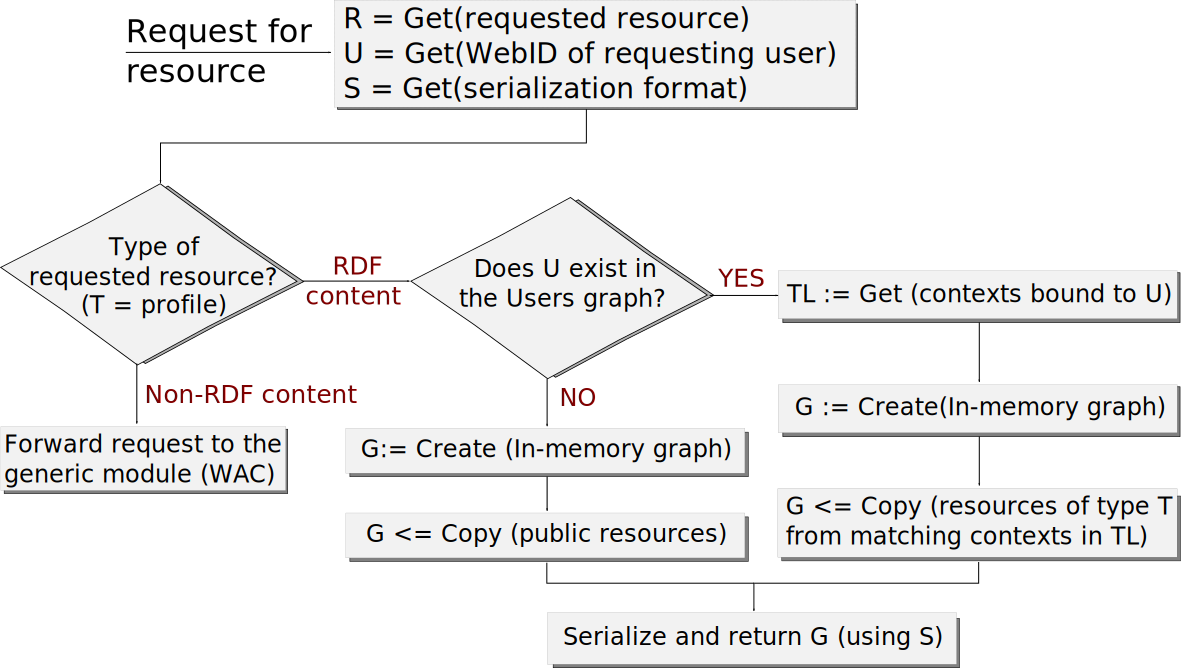
\includegraphics[width=270px]{img/algorithm-matching.pdf}
        \caption{Algorithme d'appariement contextuel.}
        \label{fig:context_matching_fr}
  \end{center}
\end{figure}

%The information contained in the \textit{Request} includes the type of the requested resource (T), the WebID of the requester (U) and the data serialization format (S) for the response (e.g. Turtle, RDF/XML, N3, etc.). At this point, we assume that the requesting user has already been authenticated at the moment of the request. If the user has not been authenticated, only the public view of the requested resource is returned.\\
Les informations contenues dans la demande inclut le type de la ressource demandée (T), le WebID du demandeur (U) et le format de sérialisation de données (S) pour la réponse (par exemple, Turtle, RDF / XML, N3, etc). À ce stade, nous supposons que l'utilisateur demandeur a déjà été authentifié au moment de la demande. Si l'utilisateur n'a pas été authentifié, seule la vue publique de la ressource demandée est renvoyée.\\


%The following step of the algorithm is to lookup the requester in the graph of users belonging to the resource owner. If there is no match, the requester receives only the public view of the requested resource. Otherwise, all contexts assigned to the requester's WebID are extracted, and a list of all contexts URIs (TL) is created.\\
L'étape suivante de l'algorithme est de rechercher le demandeur dans le graphique des utilisateurs appartenant au propriétaire de la ressource. Si aucune correspondance n'est trouvée, le demandeur ne reçoit que la vue publique de la ressource demandée. Sinon, tous les contextes affectés au WebID du demandeur sont extraites, et une liste de tous les contextes URI (TL) est crée.\\


%The next step is to create a temporary, in-memory graph (G), to store only the resources matching the requester's access policies. This graph will only be used during the processing of the algorithm, to hold the contents of the reply.\\
L'étape suivante consiste à créer un graphe temporaire en mémoire (G), afin de conserver uniquement les ressources correspondant à la politique d'accès du demandeur. Ce graphe ne sera utilisé que pendant le traitement de l'algorithme, afin de maintenir le contenu de la réponse.\\


%Once the graph has been created, it is time to copy all resources belonging to the list of contexts (TL), and which correspond to the type of the request (e.g. a profile, a wall, a conversation, etc.).\\
Une fois que le graphe a été créé, il est temps de copier toutes les ressources appartenant à la liste des contextes (TL), et qui correspondent au type de la demande (par exemple, un profil, un mur, une conversation, etc).\\


%Finally, the graph (G) is serialized in the requested format (S) before being returned to the requesting user (U). As soon as the contents of (G) have been sent through HTTP(S), the graph is destroyed and memory is freed.
Enfin, le graphe (G) est mis en forme sur la base de la sérialisation demandée (S) avant d'être renvoyé à l'utilisateur demandeur (U). Dès que le contenu de (G) a été envoyé via HTTP(S), le graphe est détruit et la mémoire est libérée.

\addcontentsline{toc}{subsection}{Le moteur de la surveillance des relations}
\subsection*{Le moteur de la surveillance des relations}
%The \textit{Relationship Monitor} engine (RM) is tasked to analyse the dynamicity of relationships between two given users, in order to either provide notifications for potential privacy issues that may arise when disclosing information, or it may even modify existing access control policies for incoming requests (if so configured). The RM applies to two distinct types of actions. First, for assigning context labels when disclosing information, and second for handling a request for a resource.\\
Le moteur de surveillance des relations (Relationship Monitor - RM) est chargé d'analyser le caractère dynamique des relations entre les deux utilisateurs donnés, afin de fournir soit des notifications pour les éventuels problèmes de la vie privée qui peuvent surgir lors de la divulgation d'information, ou il peut même modifier les politiques de contrôle d'accès existants pour les requêtes entrantes (s'il est configuré pour). Le RM s'applique à deux types distincts d'actions. Tout d'abord, pour attribuer des étiquettes de contexte lors de la divulgation d'informations, et la seconde pour le traitement d'une demande de ressource.\\


%When a user intends to limit the audience for some of his/her private information (e.g. religious views, sexual orientation, etc.), he/she can assign one or more context labels to the information that is to be protected, as well as to the audience in order to indicate who can access the information. During this labelling process, the RM analyses user interaction data from the Relationship History database (Figure~\ref{fig:acs_architecture}), corresponding to the selected audience. Typical examples of user interactions include sharing a picture within a specific context (i.e. \verb+#closefriends+), explicitly changing a user's proximity level, excluding a user from a given context (without permanently removing him/her) when sharing a resource, the number of times users exchange messages (as a function of time), etc.\\
Quand un utilisateur a l'intention de limiter l'audience de certaines de ses informations personnelles (par exemple, opinions religieuses, l'orientation sexuelle, etc), il peut assigner une ou plusieurs étiquettes de contexte à l'information qui doit être protégée, ainsi que pour le public afin d'indiquer qui peut accéder à l'information. Au cours de ce processus d'étiquetage, la RM analyse les données d'interaction de l'utilisateur à partir d'un historique des relations (Relationship History database - Figure~\ref{fig:acs_architecture_fr}), correspondant à l'auditoire sélectionné. Des exemples typiques d'interactions entre les utilisateurs comprennent le partage d'une image dans un contexte spécifique (par exemple \verb+#closefriends+), changer explicitement le niveau de proximité d'un utilisateur, exclure un utilisateur à partir d'un contexte donné (sans l'enlever définitivement) lors du partage d'une ressource, combien de fois les utilisateurs échangent des messages (en fonction du temps), etc.\\


%Based on the interactions in Relationship History database, the RM may alert the user (i.e. provide visual indications) to a possible change in their relationship. For instance, a warning message may appear if the resource owner is in the process of assigning a context label (which corresponds to a specific proximity level) to a user which is in a more distant proximity level.\\
Basé sur les interactions dans le historique des relations, le RM peut alerter l'utilisateur (par exemple fournir des indications visuelles) à un éventuel changement dans leur relation. Par exemple, un message d'avertissement peut apparaître si le propriétaire de la ressource est en cours d'attribution d'une étiquette de contexte (ce qui correspond à un niveau de proximité spécifique) à un utilisateur qui se trouve dans un niveau de proximité plus lointain.\\


%The algorithm behing the RM's decision making process can be seen in Figure~\ref{fig:algorithm_rme}.\\
L'algorithme derriere le processus de prise de décision de la RM peut être vu dans la Figure~\ref{fig:algorithm_rme_fr}.\\

\begin{figure}[h]
  \begin{center}
    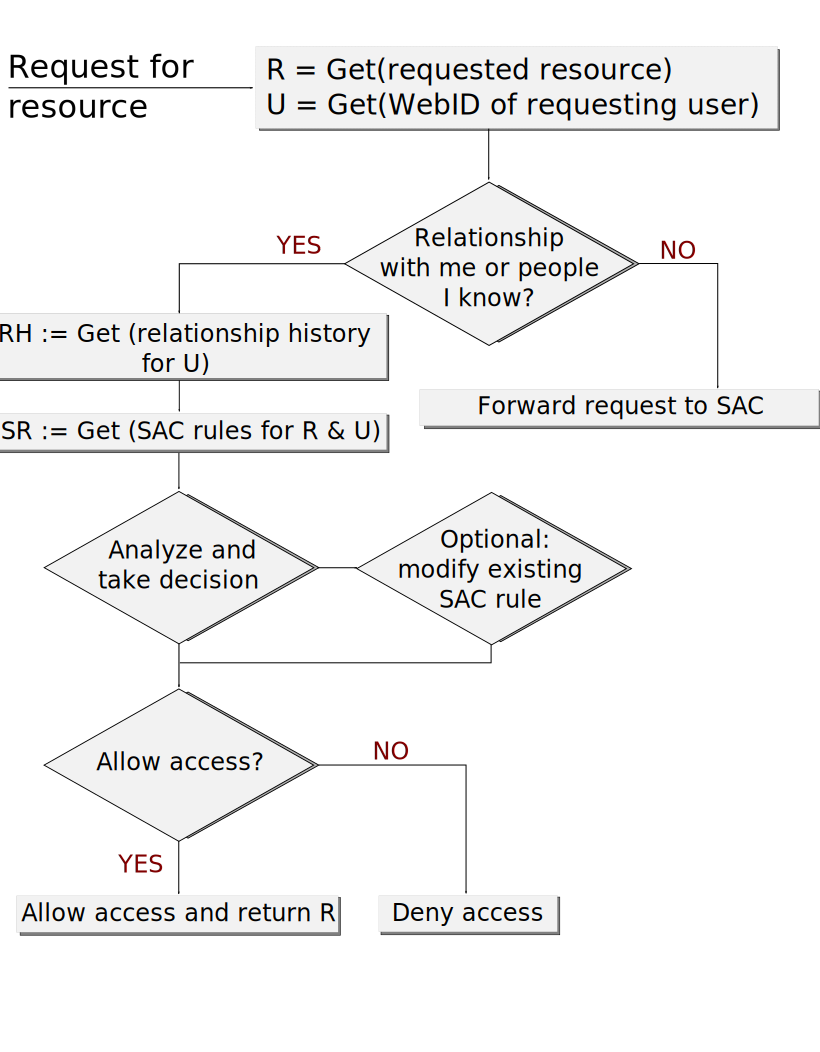
\includegraphics[width=270px]{img/algorithm-rme.pdf}
        \caption{Le processus de la prise de décision du RM.}
        \label{fig:algorithm_rme_fr}
  \end{center}
\end{figure}

%The information contained in the \textit{Request} includes the requested resource (R) and the WebID of the requester (U). At this point, we also assume that the requesting user has already been authenticated at the moment of the request. If the user has not been authenticated, the process will consider the user to be \textit{undetermined} (i.e. anyone with public access).\\
Les informations contenues dans la demande comprend la ressource demandée (R) et le WebID du demandeur (U). À ce stade, nous supposons également que l'utilisateur demandeur a déjà été authentifié au moment de la demande. Si l'utilisateur n'a pas été authentifié, le processus considèrent que l'utilisateur soit indéterminée (i.e. à toute personne ayant accès public).\\


%The following step is to decide if the user in question has any relationships with the resource owner or people known by the resource owner. This step is achieved by querying the Relationship History database to find occurrences of interactions between the requester and the resource owner, or by searching if the requester is friends with the resource owner or one of the resource owner's friends.\\
L'étape suivante consiste à décider si l'utilisateur en question a des relations avec le propriétaire de la ressource ou des personnes connues par le propriétaire de la ressource. Cette étape est effectuée en interrogeant la base de données contenant l'historique des relations pour trouver les occurrences d'interactions entre le demandeur et le propriétaire de la ressource, ou en recherchant si le demandeur est ami avec le propriétaire de la ressource ou l'un des amis du propriétaire de la ressource.\\


%If the two users have previously interacted with each other, a graph (RH) containing the list of interactions will be created. Additionally, all static access control rules corresponding to the user (U) and resource (R) will be imported from the policies database and stored in a new graph (SR).\\
Si les deux utilisateurs partagent un historique des relations, un graphe (RH) contenant la liste des interactions sera créé. De plus, toutes les règles statiques de contrôle d'accès correspondant à l'utilisateur (U) et ressources (R) seront importées à partir de la base de données des politiques et stockés dans un nouveau graphe (SR).\\


%Next, based on the the contents of (RH) and (SR), the system will analyse an decide on a course of action. If the data from (RH) is found to be heavily conflicting with the rules in (SR) and if the RM engine is operating in \textit{unsupervised mode}, the system may optionally modify existing SAC rules. For example, if the requester was deemed to have changed proximity distance either through an evolution of his/her relationship towards the resource owner, or because the resource owner explicitly modified the user's proximity distance, the system may be able to reflect this change in the SAC rules.\\
Ensuite, basé sur le contenu de (RH) et (SR), le système va analyser et décider d'un plan d'action. Si les données de (RH) se trouve être fortement contradictoires avec les règles (SR) et si le moteur RM fonctionne en mode sans surveillance, le système peut éventuellement modifier les règles SAC existants. Par exemple, si le demandeur est réputé avoir changé sa distance de proximité, soit par une évolution de sa relation envers le propriétaire des ressources, soit parce que le propriétaire de la ressource a explicitement modifié la distance de proximité de l'utilisateur, le système peut être en mesure de refléter ce changement dans le règles SAC.\\


%Once the final decision is made, the RM engine will either grant access or deny access to the requested resource.
Une fois que la décision finale est prise, le moteur RM va accorder ou refuser l'accès à la ressource demandée.


\addcontentsline{toc}{section}{Validation de nos travaux de recherche}
\section*{Validation de nos travaux de recherche}
%A truly decentralized social Web application, based on Semantic Web technologies, requires several key components. It must be able to offer decentralized user identity, secure authentication, semantic data storage, to apply Create-Read-Update-Delete (CRUD) operations to resources, to offer increased privacy through access control, and most importantly, to be interoperable with other applications in terms of data exchange (e.g. content sharing, messaging, activity notifications, etc.).
Une application Web véritablement décentralisée, basée sur les technologies du Web sémantique, nécessite plusieurs éléments clés. Elle doit être en mesure d'offrir une identité décentralisée pour l'utilisateur, d'offrir une authentification sécurisée, du stockage de données sémantique, appliquer des opérations Create-Read-Update-Delete (CRUD) aux ressources, d'offrir plus d'intimité grâce au contrôle d'accès, et surtout, d'être interopérable avec d'autres applications en termes d'échange de données (par exemple, le partage de contenu, la messagerie, les notifications d'activité, etc).

\addcontentsline{toc}{subsection}{MyProfile}
\subsection*{MyProfile}
%MyProfile project is a reflection of all efforts we have made over the course of this thesis. It intends to provide to users the privacy they deserve for the data they produce and own. It offers a unified user account, which centralizes the user's data and puts it under the user's control, and also on a device the user controls. It is a radical change from the \textit{walled gardens} of today's Web, where data are trapped in \textit{silos}.\\
Le projet de MyProfile est le reflet de tous les efforts que nous avons faits au cours de cette thèse. Il vise à fournir aux utilisateurs la la vie privée qu'ils méritent pour les données qu'ils produisent et détiennent. Il dispose d'un compte d'utilisateur unifiée, qui centralise les données de l'utilisateur et le met sous le contrôle de l'utilisateur, et également sur un dispositif appartenant à l'utilisateur. C'est un changement radical par rapport aux \textit{jardins clos} du Web d'aujourd'hui, où les données sont piégées dans des \textit{silos}.\\


%The platform also offers other services that do not require a local profile. Any user is able to \textit{view} his/her profile data in a friendlier and attractive way. While viewing the profile data, the platform displays the user's list of known people (i.e. friends), some basic information for each friend (e.g. full name, nickname, email, blog), as well as a text mention in case the relationship is bidirectional (i.e. "Has you as friend.").\\
La plate-forme propose également d'autres services qui ne nécessitent pas un profil local. N'importe quel utilisateur peut visualiser ses données de profil d'une manière conviviale et attrayante. Lors de l'affichage des données de profil, la plate-forme affiche la liste des utilisateurs de gens connus (i.e. amis), quelques informations de base pour chaque ami (par exemple nom, prénom, pseudo, email, blog), ainsi qu'une mention de texte au cas où la relation est bidirectionnelle (i.e. "vous a comme ami.»).\\


%Once authenticated, additional functionalities become available. For example, users can post messages to a public \textit{wall}, which is a common place for all users to write about news, events, social updates, etc. Users can also \textit{subscribe} to local services in order to have their own private wall, which is only available to their list of known people. Subscribing also allows users to send and receive private messages, as well as notifications when other users have posted something on their private wall.\\
Une fois authentifié, des fonctionnalités supplémentaires sont disponibles. Par exemple, les utilisateurs peuvent envoyer des messages sur un mur public, qui est un lieu commun pour tous les utilisateurs à écrire à propos de nouvelles, des événements sociaux, des mises à jour, etc. Les utilisateurs peuvent également s'abonner à des services locaux afin d'avoir leur propre mur privé, ce qui est disponible uniquement à leur liste de personnes connues. S'abonner permet également aux utilisateurs d'envoyer et de recevoir des messages privés, ainsi que des notifications lorsque d'autres utilisateurs ont posté quelque chose sur leur mur privé.\\

%The source code for MyProfile has been released under an MIT license (less restrictive compared to other open source licenses), and it is publicly available on GitHub under MyProfile\footnote{https://github.com/MyProfile/myprofile}. For portability and deployment reasons, the platform was mainly written in PHP and JavaScript. It relies on Virtuoso\footnote{http://virtuoso.openlinksw.com/} to facilitate RDF-triple storage and SPARQL queries for cached profiles. A running demo of MyProfile can be accessed at https://my-profile.eu/.
Le code source pour MyProfile a été publié sous une licence MIT (moins restrictive par rapport à d'autres licences open source), et il est accessible au public sur GitHub sous MyProfile\footnote{https://github.com/MyProfile/myprofile}. Pour des raisons de portabilité et de déploiement, la plate-forme a été principalement écrit en PHP et JavaScript. Elle s'appuie sur un système de stockage de triplets RDF basé sur Virtuoso\footnote{http://virtuoso.openlinksw.com/}, qui offre des requêtes SPARQL pour les profils mis en cache. Une démo fonctionnelle de MyProfile peut être consultée à https://my-profile.eu/.

\addcontentsline{toc}{subsection}{Authentification WebID}
\subsection*{Authentification WebID}
%WebID-TLS authentication plays a crucial role in MyProfile. On one hand it allows any authenticated user to post messages on walls or contact other people, regardless if they have a local account or not. On the other hand, local users that have been authenticated can also easily update their profiles, issue new certificates or manage their friends.\\
Authentification WebID-TLS joue un rôle crucial dans MyProfile. D'une part, il permet à tout utilisateur authentifié d'envoyer des messages sur les murs ou contacter d'autres personnes, peu importe si elles ont un compte local ou non. D'autre part, les utilisateurs locaux qui ont été authentifiés peuvent aussi facilement mettre à jour leurs profils, émettre de nouveaux certificats ou de gérer leurs amis.\\


%There exists two different WebID-TLS authentication approaches, either perform the WebID-TLS verification locally, or use a third party WebID-TLS authentication service. We have developed two libraries, written in PHP, which cover both approaches. The libraries have been released under the MIT license, and are publicly available on GitHub under WebIDauth\footnote{https://github.com/organizations/WebIDauth}. In the following subsections we will describe both libraries, as well as how the Web server must be configured to offer WebID-TLS authentication.
Il existe deux approches d'authentification WebID-TLS différentes. Ils peuvent soit effectuer la vérification WebID-TLS localement ({WebIDauth}) ou utiliser un autre service tiers d'authentification WebID-TLS (WebIDDelegatedAuth). Nous avons développé deux bibliothèques, écrites en PHP, qui couvrent les deux approches. Les bibliothèques ont été publiées sous la licence MIT, et sont accessibles au public sur GitHub sous WebIDauth\footnote{https://github.com/organizations/WebIDauth}. Dans les paragraphes qui suivent, nous allons décrire les deux bibliothèques.

\subsubsection*{WebIDauth}
%Local authentication can be achieved by relying on \textit{WebIDauth}, a PHP library implementing WebID-TLS. Its particularity resides in the fact that it allows users to request a \textit{verbose} authentication process, which is useful when debugging a faulty certificate or a user profile.\\
L'authentification locale peut être réalisée en s'appuyant sur WebIDauth, une bibliothèque PHP qui implémente WebID-TLS. Sa particularité réside dans le fait qu'il permet aux utilisateurs de demander un processus d'authentification verbeux, ce qui est utile lors du débogage d'un certificat défectueux ou un profil d'utilisateur.\\


%WebIDauth can operate in two modes. In the first mode, its task is to perform WebID-TLS authentication and simply return either \textit{true} or \textit{false}, depending whether the user was successfully authenticated or not. This mode is intended to be used as an authentication method for a local application, usually coupled with a user session. However, operating in this mode also implies configuring the Web server to run over HTTPS, adding to the expenses of hosting the local application by having to buy a server certificate.\\
WebIDauth peut fonctionner dans deux modes. Dans le premier mode, sa tâche consiste à effectuer une authentification WebID-TLS et il suffit de retourner \textit{Vrai} ou \textit{Faux}, selon si l'utilisateur a été authentifié avec succès ou non. Ce mode est prévu pour être utilisé comme un procédé d'authentification pour une application locale, généralement associée à une session d'utilisateur. Cependant, fonctionnant dans ce mode implique également la configuration du serveur Web pour exécuter via HTTPS, en ajoutant aux dépenses de l'hébergement de l'application locale la nécessité acheter un certificat de serveur.\\


%In the second operation mode, WebIDauth can be used as a Relying Party, a third-party service that provides a WebID-TLS authentication endpoint for Web applications that cannot perform the authentication process themselves. There are several advantages to using a Relying Party service. For instance, it drastically reduces the complexity of having to set up the Web server to allow WebID-TLS authentication. Additionally, the service provider (local application) may not require HTTPS, therefore the owners do not need to pay for a server certificate.
Dans le deuxième mode de fonctionnement, WebIDauth peut être utilisé comme un service tiers qui fournit un point d'accès authentification WebID-TLS pour les applications Web qui ne peuvent pas effectuer le processus d'authentification eux-mêmes (essentiellement un RP). Dans le deuxième mode de fonctionnement, WebIDauth peut être utilisé comme un service tiers qui fournit un point d'accès authentification WebID-TLS pour les applications Web qui ne peuvent pas effectuer le processus d'authentification eux-mêmes (essentiellement un RP). Il ya plusieurs avantages à utiliser un service tiers. Par exemple, il réduit considérablement la complexité d'avoir à configurer le serveur Web pour permettre l'authentification WebID-TLS. En outre, le prestataire de service (application locale) n'a pas à exiger HTTPS, donc les propriétaires n'ont pas besoin de payer pour un certificat de serveur.


\subsubsection*{WebIDDelegatedAuth}
%Delegated WebID-TLS authentication is the process of relying on a third-party service to perform the authentication, and then redirect the user back to the Service Provider, as seen Section~\ref{sec:webid-tls_delegated_auth}. This is currently the default operation mode for MyProfile. The WebIDDelegatedAuth library was created so that Service Providers can offer WebID-TLS authentication in case they are not capable of offering local authentication, or they do not operate over HTTPS. Let us now explore each step of the process.\\
L'authentification WebID-TLS délégué est le processus de s'appuyer sur un service tiers pour effectuer l'authentification, puis rediriger l'utilisateur vers le fournisseur de services. Ce n'est pas le mode de fonctionnement par défaut pour MyProfile. La bibliothèque WebIDDelegatedAuth a été crée afin que les fournisseurs de services puissent offrir une authentification WebID-TLS dans le cas où ils ne sont pas capables d'offrir une authentification locale, ou ils ne fonctionnent pas via HTTPS. Examinons maintenant chaque étape du processus.\\


%First, the user clicks a login button on the Service Provider (i.e. https://my-profile.eu) and is redirected to the Relying Party (i.e. https://auth.my-profile.eu), thus triggering the authentication process. The Service Provider also appends a variable to the redirection URI, containing the Service Provider's URI: \textit{https://auth.my-profile.eu/?authreqissuer=https://my-profile.eu}.\\
Tout d'abord, l'utilisateur clique sur un bouton de connexion sur le fournisseur de services (i.e. https://my-profile.eu) et est redirigé vers le RP (i.e. https://auth.my-profile.eu), déclenchant ainsi le processus d'authentification. Le fournisseur de service ajoute également une variable à l'URI de redirection, contenant l'URI du fournisseur de services: \textit{https://auth.my-profile.eu/?authreqissuer=https://my-profile.eu}.\\


%Next, the Relying Party uses WebIDauth to perform WebID-TLS authentication. If the user has been successfully authenticated, the Relying Party prepares the redirection request, appending additional arguments to the redirection URI, namely the \textit{webid}, \textit{ts}, \textit{referrer} and \textit{sig}, with the following meanings:
Ensuite, le RP utilise la bibliothèque WebIDauth pour effectuer une authentification WebID-TLS locale. Si l'utilisateur a été authentifié avec succès, le RP prépare la demande de redirection, en ajoutant des arguments supplémentaires à l'URI de redirection, comme le \textit{webid}, \textit{ts}, \textit{referrer} et \textit{sig}, qui ont les significations suivantes:

\begin{itemize}
\item \verb+webid+ - WebID: https://my-profile.eu/people/barry/card\#me.
\item \verb+ts+ - horodatage: 2013-05-22CEST16\%3A54\%3A04\%2B02\%3A00
\item \verb+referrer+ - https://auth.my-profile.eu
\item \verb+sig+ - signature: hR5cv9gPn.....MxBbSdq7f.
\end{itemize}

\addcontentsline{toc}{subsection}{Espaces de données personnelles basés sur RWW.I/O}
\subsection*{Espaces de données personnelles basés sur RWW.I/O}
%Offering individual data stores is an important aspect of any decentralized social application, as users must be allowed to choose where they want to host their data, as well as to have complete control over the privacy settings that apply to that data. If possible, data stores should be hosted by devices to which the user has physical access. However, for performance reasons, data stores may be located on third party servers, if users are not concerned by privacy issues.\\
Offrant des espaces individuels de données est un aspect important de toute application sociale décentralisée. Les utilisateurs doivent être autorisés à choisir où ils veulent héberger leurs données, ainsi que d'avoir un contrôle complet sur les paramètres de confidentialité qui s'appliquent à ces données. Si possible, les espaces données doivent être hébergés sur des dispositifs auxquels l'utilisateur a un accès physique. Cependant, pour des raisons de performances, les espaces de données peuvent être situés sur des serveurs tiers, si les utilisateurs ne sont pas concernés par les questions de confidentialité.\\


%RWW.I/O stands for \textit{Read-Write-Web Input/Output} and it operates under the assumption that users require a personal data store, where different applications can store data about and for the user, and where data are equally available between applications. The advantage is that different applications can reuse the same data, to offer different functionalities. For example, a contact management application can pull data from the user's profile and modify it at the user's request. The modifications are instantly reflected in the user's profile the next time someone accesses the profile.\\
RWW.I/O signifie \textit{Read-Write-Web Input/Output} et fonctionne sous l'hypothèse que les utilisateurs ont besoin d'un espace de données à caractère personnel, où les différentes applications peuvent stocker des données sur et pour l'utilisateur, et pour lesquels des données sont également disponibles entre les applications. L'avantage est que les différentes applications peuvent réutiliser les mêmes données, afin d'offrir des fonctionnalités différentes. Par exemple, une application de gestion de contacts peut extraire des données à partir du profil de l'utilisateur et de le modifier à la demande de l'utilisateur. Les modifications sont immédiatement reflétées dans le profil de l'utilisateur la prochaine fois que quelqu'un accède au profil.\\


%Being invited to work with Sir Tim Berners-Lee on access control for the the Semantic Web at the Massachusetts Institute of Technology, has allowed me to develop a Linked Data personal data store platform that implements the WAC~\cite{hollenbach2009using} ontology. The platform supports full Create-Read-Update-Delete (CRUD) operations, following the REST standards. Documents and directories can be created by performing HTTP requests such as POST, PUT and MKCOL (i.e. new directories), following the requirements we presented at the beginning of the chapter. The \textit{Content-Type} HTTP header plays a central role to interpreting the requests and deciding whether to store data as triples or as binary files. As RWW.I/O is not intended to be a fully-fledged cloud service, only a handful of content types are supported (e.g. text/turtle, text/n3, application/rdf+xml, application/json, text/html, image/jpg, image/png).\\
Être invité à travailler avec Sir Tim Berners-Lee sur le contrôle d'accès pour le Web Sémantique au Massachusetts Institute of Technology, m'a permis de commencer le développement de RWW.I/O tandis que la mise en œuvre de l'ontologie WAC. La plate-forme prend en charge les opérations complètes Create-Read-Update-Delete (CRUD), suivant le standard REST. Documents et répertoires peuvent être créés en effectuant des requêtes HTTP tels que POST, PUT et MKCOL (nouveaux répertoires), suivant les besoins, nous avons présenté au début de ce document. L'en-tête HTTP \textit{Content-Type} joue un rôle central pour interpréter les demandes et décider de stocker des données comme des triplets ou sous forme de fichiers binaires. Comme RWW.I/O n'est pas destiné à être un service de cloud à part entière, seule une poignée de types de contenu sont pris en charge (e.g. text/turtle, text/n3, application/rdf+xml, application/json, text/html, image/jpg, image/png).\\


%The code is written in PHP, Python and JavaScript, and is publicly available under an MIT license on Github at
Le code est écrit en PHP, Python et JavaScript, et est accessible au public sous une licence MIT sur Github à \textbf{rww.io}\footnote{https://github.com/deiu/rww.io}.


\addcontentsline{toc}{section}{Conclusions}
\section*{Conclusions}
%At the beginning of this thesis we set out to identify which are the key components that would help us achieve true data ownership and interoperability for the next-gen social Web. While decentralisation is the most important factor of the equation, our model would not work unless true interoperability is achieved. For this reason, we decided to use Semantic Web technologies, as they provide true interoperability as well as helping represent data in a way that cannot be confusing or misleading.\\
Au début de cette thèse, nous avons commencé à identifier quels sont les éléments clés qui pourraient nous aider à parvenir à une véritable propriété des données et l'interopérabilité pour le Web social de prochaine génération. Si la décentralisation est le facteur le plus important de l'équation, notre modèle ne fonctionne que si une véritable interopérabilité est obtenue. Pour cette raison, nous avons décidé d'utiliser les technologies du Web sémantique, car elles offrent une véritable interopérabilité ainsi que d'aider représenter des données d'une manière qui ne peut pas prêter à confusion ou induire en erreur.\\


%During this thesis we have contributed to three different research topics, ranging from decentralized identity to authentication and access control. To validate our contributions to the research world, we have participated in the standardization process of WebID and WebID-TLS at the World Wide Web Consortium (W3C), which has allowed us to obtain immediate feedback from experts all around the world.\\
Au cours de cette thèse, nous avons contribué à trois thèmes de recherche différents, allant de l'identité décentralisée  à l'authentification et au contrôle d'accès. Pour valider nos contributions dans le monde de la recherche, nous avons participé au processus de standardisation du WebID et WebID-TLS au sein du World Wide Web Consortium (W3C), qui nous a permis d'obtenir des commentaires immédiats de la part des experts du monde entier.\\


%Furthermore, we were able to translate our research results into working services and applications, which are currently used as base references for work in this domain. All our implementation efforts consist of open source software, publicly available on GitHub with an MIT license.
Enfin, nous avons réussi à matérialiser nos résultats de recherche en services et applications qui sont actuellement utilisés comme références de base pour les travaux dans ce domaine. Tous nos efforts de mise en œuvre consistent en des logiciels open source, disponibles au public sur GitHub avec une licence MIT.

\clearpage
